\chapter{Conclusiones}

%%RESUMEN E INTRODUCCIÓN

En este Proyecto Fin de Grado se ha desarrollado un sistema de préstamos 
descentralizado basado en la red \gls{ethereum}. 
Tras el desarrollo se pueden llegar a las siguientes conclusiones:
\begin{itemize}
     \item Se puede afirmar que se ha obtenido 
una aplicación capaz de conectarse con una red \gls{blockchain} y de realizar 
transacciones en ella.

Gracias al registro de estas transacciones y cierta lógica aplicada 
a esta información, se puede componer un sistema de creación y control de préstamos 
digitales en el que el contrato de nuevos préstamos queda totalmente automatizado.

     \item Es posible unificar todas las herramientas de gestión dentro de la una interfaz de 
usuario cubriendo todas las conexiones necesarias con la red de \gls{ethereum} 
y capaz de ordenar la ejecución en la red las operaciones necesarias para la 
gestión de un sistema de préstamos digitales.

     \item Aunque para un sistema aplicado en la vida real hiciera falta 
     la implementación de distintos desarrollos, los \glspl{smartcontract} 
     desplegados en la red definen correctamente la lógica 
     aplicada a la información necesaria para la realización de préstamo.

     \item El correcto registro de esta información en la red \gls{blockchain} 
     proporciona al sistema las características de seguridad, inmutabilidad y 
     veracidad necesarias para un sistema de esta índole.

     \item Exite un plan de validación que verifica las capacidades descritas 
     para este sistema.

     \item Tras un estudio del impacto social se puede concluir que la adopción 
     de tecnologías \gls{defi} y \gls{smartcontract} tiene el potencial de transformar
     el acceso a servicios financieros y dependiendo del uso que se de a esta 
     tecnología se puede aumentar o disminuir la inclusión financiera.
\end{itemize}




\section{Trabajo futuro}

En el desarrollo de este proyecto se ha podido comprobar que un sistema de prestamos
descentralizado es posible, pero, para que un proyecto como este llegue a una situación
de producción real es necesario realizar una serie de desarrollos para cumplir con 
necesidades básicas en un sistema de préstamo real.

Se considera la más importante la adopción de garantías de impago, esta carencia del 
proyecto se tiene en cuenta en el Caso de uso futuro \hyperlink{cu:garantia}{CU12} :  Garantía de devolución en 
caso de impago,
aunque actualmente el sistema sea capaz de penalizar los impagos, no se garantiza recuperar
el capital prestado, para ello se pueden desarrollar dos casos de uso:
\begin{itemize}
     \item Creación de sistema de colaterales: en un futuro será de obligado 
     cumplimiento que el usuario que solicite un prestamo añada al sistema 
     alguna garantía, la cual puede estar en forma de \gls{nft}, y en caso 
     de que el usuario se declare en situación de impago, este \gls{nft} pasaría 
     automaticamente a ser propiedad del sistema
     \item Creación de sistema de avales: En situaciones en los que el usuario 
     no pueda añadir esa garantía o colateral se podrá añadir al contrato un tercero 
     capaz de añadir un colateral al contrato e incluso encargarse de las cuotas en 
     caso de que el usuario principal no lo haga
\end{itemize}

El nuevo sistema de garantías también debera incluir un sistema de validación de 
solvencia, tal y como se habla en el Caso de uso futuro \hyperlink{cu:garantia}{CU14}, lo que aportará 
mayor solided a la garantía de devolución.

Durante los tests de funcionamiento del sistema se pudo comprobar las ineficencias 
de código en la red. Sobretodo evitar recorrer todos los contratos existentes 
una vez al mes para comprobar si han sido pagados o no. 

Para ello el sistema se puede 
apoyar en elementos externos a la red, como una base de datos temporal en la que 
puede 
quedar reflejado cada pago de la mensualidad y mensualmente ejecutar las 
penalizaciones en la red con los contratos que no aparecen en esta base de datos,
aunque sea una base de datos externa, su uso no rompe con ninguna característica 
en las que se apoya el sistema ya que solo sería un apoyo técnico, 
manteniendo siempre 
reflejado en la red la situación financiera del sistema.

Como se pudo ver en la sección de~\ref{subsec:limitaciones-legales}, durante 
el desarrollo del proyecto, la Unión Europea abrueba un nuevo Reglamento Europeo de 
criptoactivos, por lo que para una producción real es de obligado cumplimiento 
cubrir esta normativa.

En el~\ref{op:2} se habla de que este proyecto debe contener una interfaz de usuario 
unificada, facil e intuitiva. Aunque si se ha desarrollado una interfaz unificada 
sería necesario crar una intefaz más intuitiva al usuario.

Con menos prioridad se deberán desarrollar sistemas que utilicen \gls{oraculo} 
tal y como se habla en el Caso de uso Futuro \hyperlink{cu:garantia}{CU13}, este sistema junto a la comprobación 
de solvencia económica pueden servir para una correcta definición de  los tipos de 
prestamo y condiciones disponibles en el sistema.





\section{Impactos sociales y ambientales del desarrollo de este sistema a gran escala}

La adopción masiva de un sistema de préstamos descentralizado basado en blockchain y 
contratos inteligentes podría generar importantes transformaciones en el ámbito financiero y social.
La eliminación de intermediarios permitiría un acceso más democrático a los servicios financieros,
especialmente en regiones con sistemas bancarios limitados o restrictivos.

Sin embargo, este modelo también presenta retos significativos en términos de inclusión digital,
     regulación y sostenibilidad ambiental.

\subsection{Impactos sociales}
Sin embargo,
la reducción de intermediarios no garantiza por sí sola una mayor
inclusión financiera. Su impacto social dependería de las condiciones
de acceso al crédito, de las competencias digitales de los usuarios
y de los mecanismos de protección disponibles~\cite{oecd2024defi}.

\begin{enumerate}
     \item La posibilidad de otorgar préstamos sin la necesidad de bancos tradicionales
      podría beneficiar a millones de personas no bancarizadas en economías emergentes.
       Sin embargo, la \acrfull{ocde} señala que el acceso a estos servicios dependería del
        conocimiento en el uso de criptomonedas, \gls{wallet} digitales y plataformas \gls{defi}
         y  lo que podría aumenter la brecha digital entre quienes dominan estas herramientas
          y quienes no. A demás, la \acrfull{ocde} también señala que la responsabilidad del usuario
          sobre sus propios activos dificultan la utilización de estos.
          Por tanto,
    el acceso técnico a una plataforma no equivale a una inclusión
    financiera efectiva. En el sistema desarrollado, sería necesario
    facilitar la comprensión de su funcionamiento y del uso de
    una \gls{wallet} para reducir estas barreras~\cite{oecd2024defi}.

     \item La descentralización del sistema podría entrar en conflicto con regulaciones financieras
      existentes. Gobiernos y bancos centrales podrían imponer restricciones al uso de plataformas DeFi,
       especialmente en países donde el control financiero es una herramienta de política económica.
        Además, la anonimidad en las transacciones podría plantear problemas relacionados con el
         financiamiento ilícito si no se establecen mecanismos de verificación de identidad adecuados.

     \item La automatización de los préstamos a través de contratos inteligentes podría reducir la
      demanda de intermediarios financieros, afectando a trabajadores del sector bancario y generando
       resistencia por parte de instituciones tradicionales. Sin embargo, también abriría oportunidades
        en nuevas áreas tecnológicas, creando demanda de profesionales en blockchain, ciberseguridad y
         programación de contratos inteligentes.
     \item \textbf{Acceso efectivo al crédito.}
    El BIS advierte que muchos préstamos DeFi requieren aportar
    garantías cuyo valor supera el importe solicitado. Esta
    exigencia limita su utilidad para personas que carecen de
    patrimonio previo y necesitan financiación~\cite{aramonte2022defi}.

\end{enumerate}


\subsection{Impactos ambientales}
 
\begin{enumerate}
     \item Ethereum, aunque ha reducido su impacto ambiental tras su transición de Proof of Work (\gls{pow}) a Proof of Stake (\gls{pos}),
      sigue dependiendo de una infraestructura global de nodos y validadores que consumen energía.
       A gran escala, este sistema de préstamos podría contribuir al aumento de la demanda energética de los centros de datos y redes descentralizadas,
        lo que requeriría soluciones de eficiencia energética y compensación de emisiones.
 \end{enumerate}

 Si bien un sistema de préstamos descentralizado tiene el potencial de democratizar el acceso financiero y reducir costos,
  también presenta desafíos sociales y ambientales que deben abordarse antes de una implementación a gran escala.
   Para mitigar estos impactos, sería fundamental desarrollar estrategias de educación digital y
    establecer mecanismos de regulación equilibrados para  mejorar la eficiencia energética del sistema.

 Solo con un enfoque responsable y sostenible se podrá garantizar que este tipo de innovación beneficie a la sociedad sin comprometer
  el bienestar ambiental.

\subsection{Objetivos de desarrollo sostenible. Agenda 2030}
 La Agenda 2030 para el Desarrollo Sostenible es un plan global adoptado en 2015 por los Estados Miembros de la ONU con el objetivo de erradicar la pobreza, proteger el planeta y garantizar la prosperidad para todas las personas. Para lograrlo, se establecieron 17 \gls{ods}, que abarcan áreas clave como la educación, la igualdad de género, la acción climática, la innovación y el crecimiento económico, entre otras.

Estos objetivos buscan equilibrar el desarrollo social, económico y ambiental, promoviendo un modelo sostenible que asegure el bienestar de las generaciones actuales y futuras. Además, llaman a la colaboración entre gobiernos, empresas y la sociedad civil para alcanzar metas concretas antes del año 2030.

 En la figura 4.1 se pueden ver estos objetivos:

   \begin{figure}[H]
    \centering
    \caption{Objetivos de desarrollo sostenible de la agenda europea para 2030}
    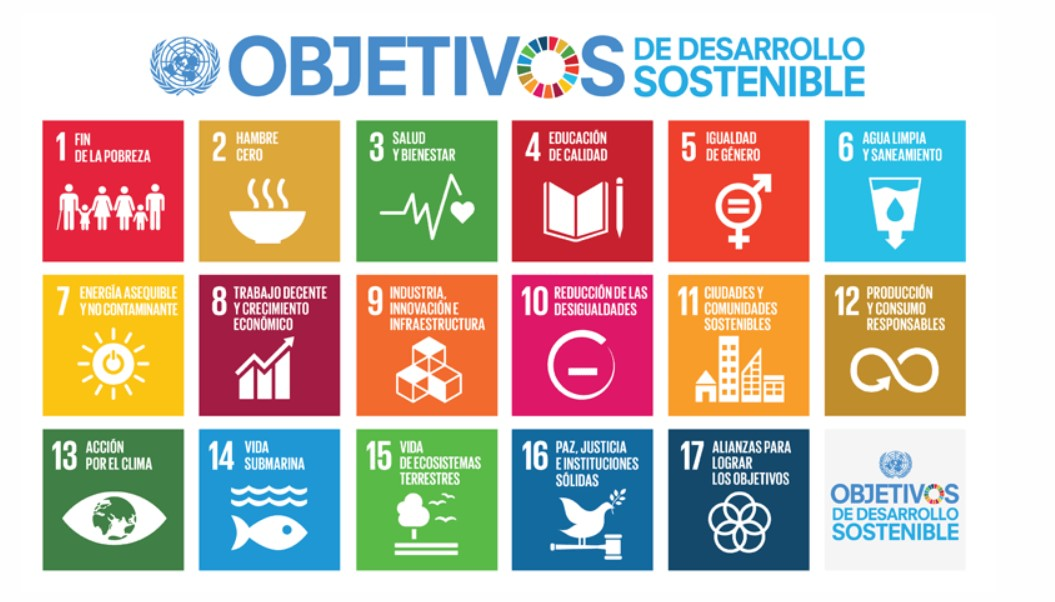
\includegraphics[width=\textwidth]{figures/2030.jpg}
    \label{fig:2030}
\end{figure}

Se puede concluir que este proyecto tiene un gran potential de influir 
positivamente en los objetivos relacionados en el ámbito financiero como los 
\gls{ods} 8 y 9 ya que supone la creación de una nueva infraestructura 
en el desarrollo de actividades económicas favoreciendo nuevas oportunidades de 
crecimiento económico.


El desarrollo de plataforma \gls{defi} tiene un gran potencial en la reducción de 
desigualdades y la aplicación de justicia social (\gls{ods} 10), la cuestión es
que el desarrollo de este potencial viene directamente correlacionado con el uso
que se le dé a esta tecnología pudiendo desarrollarse en una dirección opuesta a estos
\gls{ods}, si no se combate la brecha digital y se evita la creación de barreras articifiales pueden aumentar
por parte de los desarrolladores de esta tecnologías, 
las desigualdades y la injusticia social aumentarían todavía mas en vez de reducirse.

Algo parecido pasa con el \gls{ods} 16: la transparencia de las transacciones en un 
entorno descentralizado suponen una clara exposición de injusticias o malversaciones
realizadas en la red aunque esta característica pierde toda valided cuando se hace
un mal uso de la justicia y suceden eventos en los que se aprecia que 
\enquote{la justicia NO es igual para todos}

En el apartado ambiental (\gls{ods} 11, 12 y 13), aunque, es cierto, que tras el cambio de validación de 
bloques en la red a través de puro procesamiento y consumo eléctrico (\gls{pow})
por un sorteo en base a las aportaciones de capital en la red (\gls{pos}) se redujo
de manera drástica el consumo de electricidad, sigue habiendo otros problemas como 
la gestión de residuos de la infraestructura de la red.
Aunque volvemos a lo mismo que los apartados anteriores, siempre se puede utilizar
el aumento de productividad y capital en paliar los efectos adversos que este 
sistema incide en el ecosistema, todo depende del uso que se quiera dar a la 
tecnología.
